\section{Struttura di un documento brevettuale}

Possiamo vedere un'invenzione come una soluzione originale a un problema tecnico.\bigskip

Un brevetto è un documento sia tecnico che giuridico. Esso deve partire da una tecnica nota, individuarne un problema, fornire una soluzione descritta dettagliatamente e infine indicare le rivendicazioni. 

Le rivendicazioni:
\begin{itemize}
    \item delimitano: sintetizzano l'essenza dell'insegnamento
    \item definiscono un'astrazione della soluzione
    \item includono tutte le possibili forme concrete di realizzazione
    \item escludono le soluzioni note
\end{itemize}

\begin{figure}[h]
    \centering
    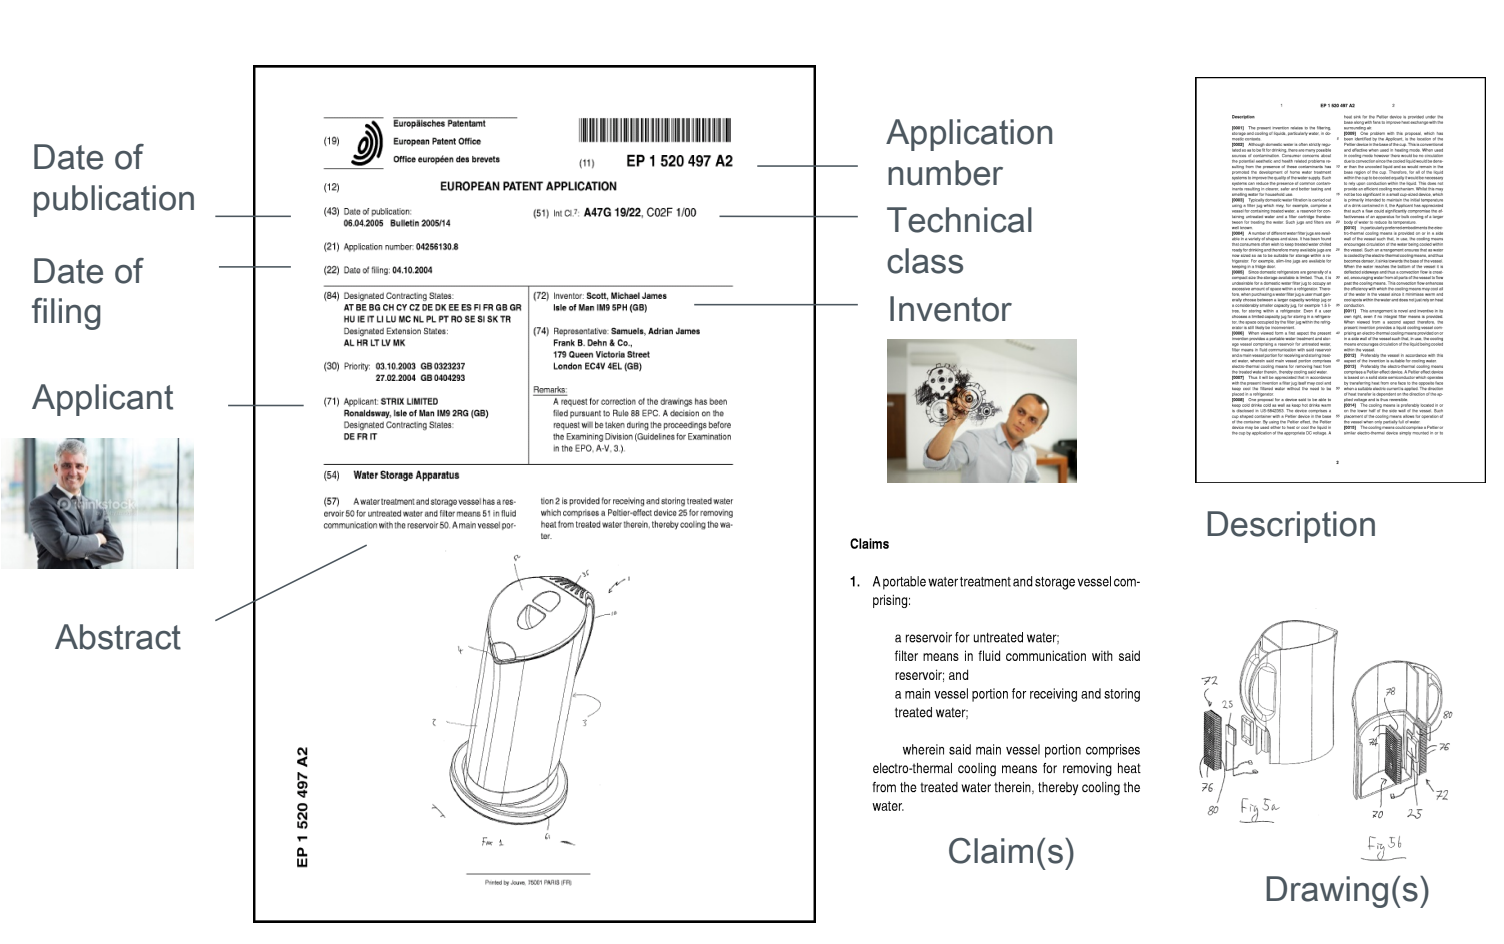
\includegraphics[width=\textwidth]{patent layout.png}
    \caption{Layout brevetto}
    \label{patent layout}
\end{figure}

Un brevetto ha normalmente una pagina di frontespizio, seguito da una parte descrittiva, da disegni e da una sezione di \textit{claims}. Molto spesso i disegni in ambito di brevettazione mettono in evidenza tramite codici numerici dettagli che vengono richiamati nel testo descrittivo. I disegni fanno parte della comunicazione dell'idea e il metodo di riferimento nel testo ai componenti rappresentati è soggetto a regolamentazione.
La struttura è mostrata in figura \ref{patent layout}.

\subsection{Il frontespizio}
Un esempio di frontespizio è mostrato in figura \ref{frontespizio}.\bigskip

\begin{figure}[!]
    \centering
    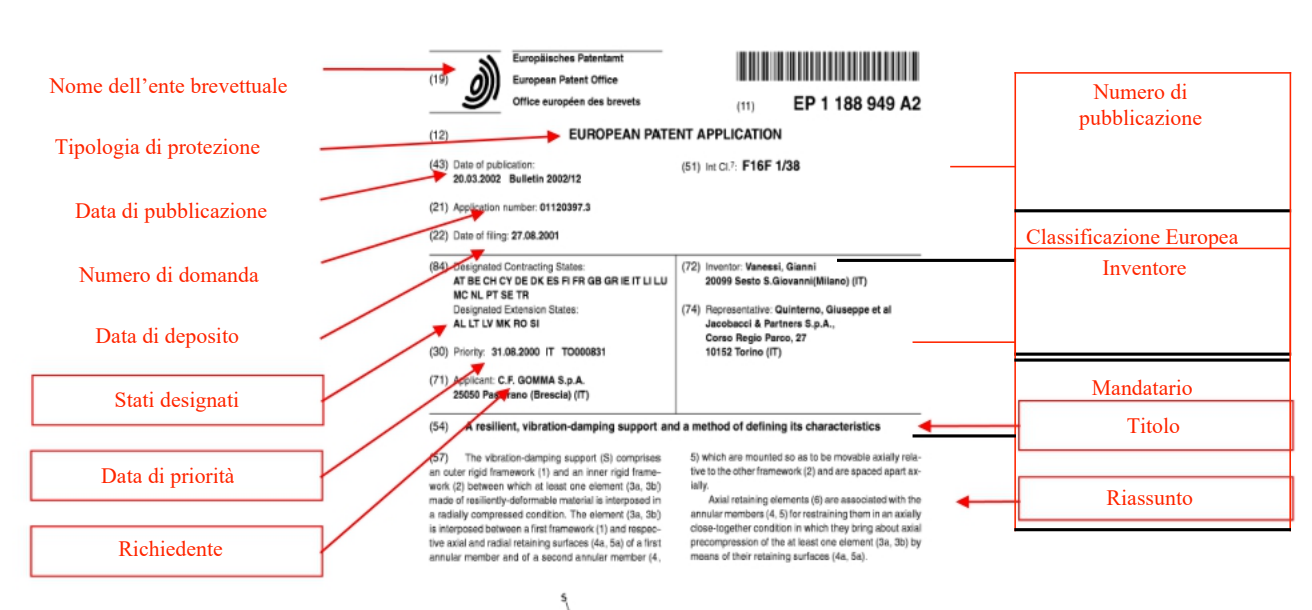
\includegraphics[width=\textwidth]{frontespizio brevetto.png}
    \caption{Frontespizio}
    \label{frontespizio}
\end{figure}

La procedura di brevettazione europea permette di scegliere in quali stati dell'UE il brevetto deve essere esteso. 

Il richiedente è colui che avrà la titolarità dei diritti, non necessariamente l'autore dell'invenzione. 

\subsection{La descrizione}
Riporta i problemi tecnici risolti dall'introduzione dell'invenzione ma è ancora una descrizione abbastanza libera e generica rispetto a quanto avviene nei \textit{claims}.

\begin{figure}[!]
    \centering
    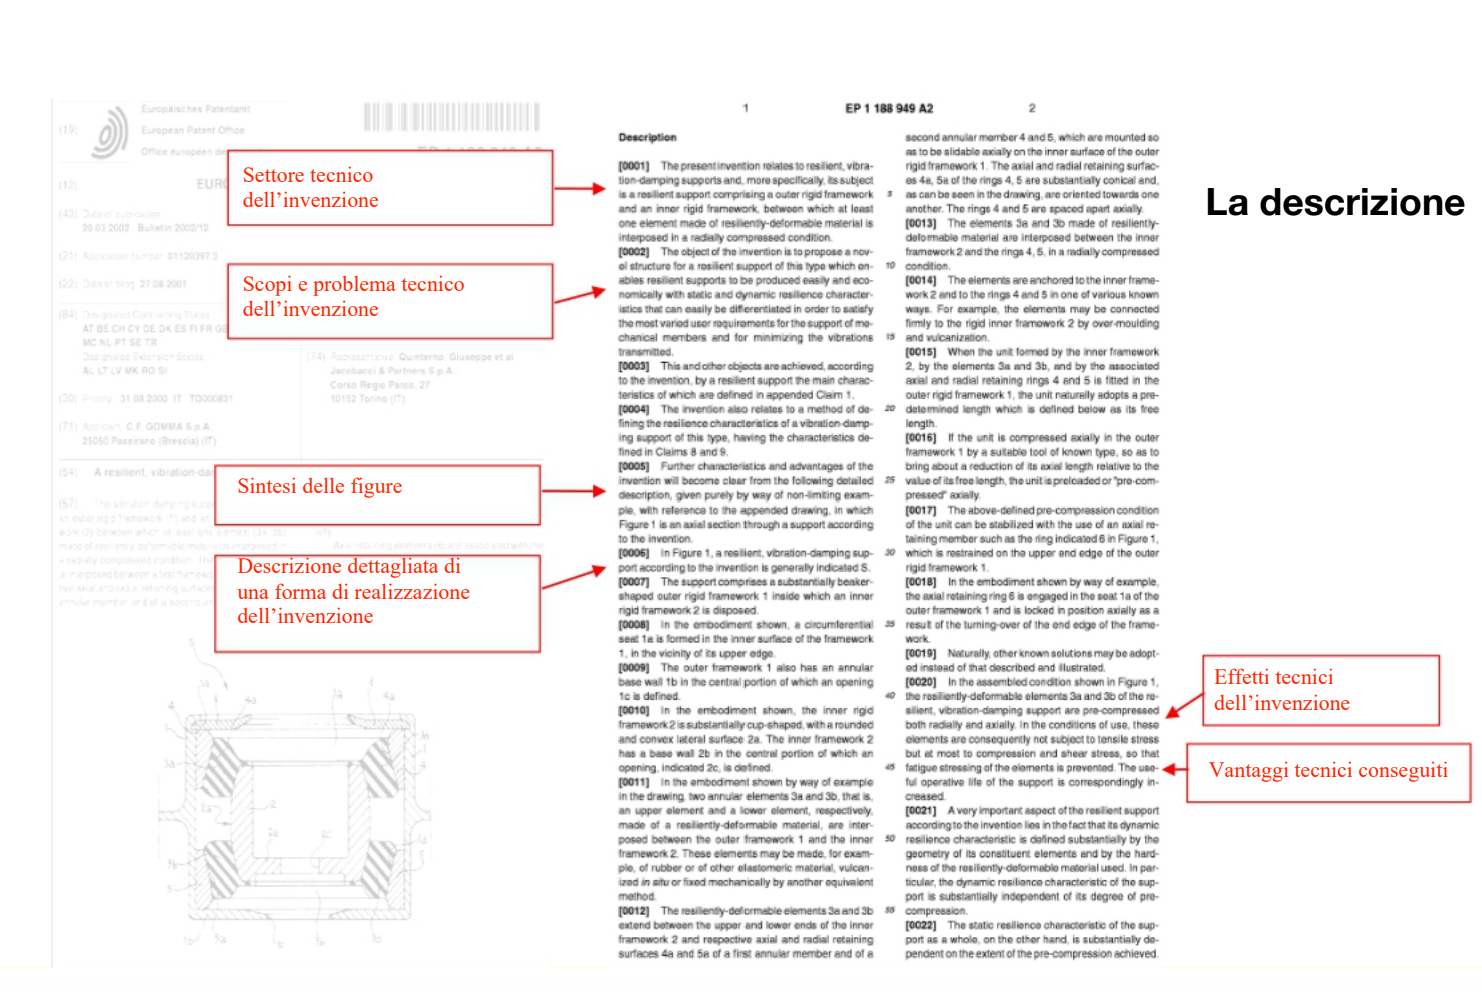
\includegraphics[width=\textwidth]{descrizione patent.png}
    \caption{Descrizione}
    \label{descrizione}
\end{figure}

\subsection{Rivendicazioni}
Vedi figura \ref{claims}

\begin{figure}[!]
    \centering
    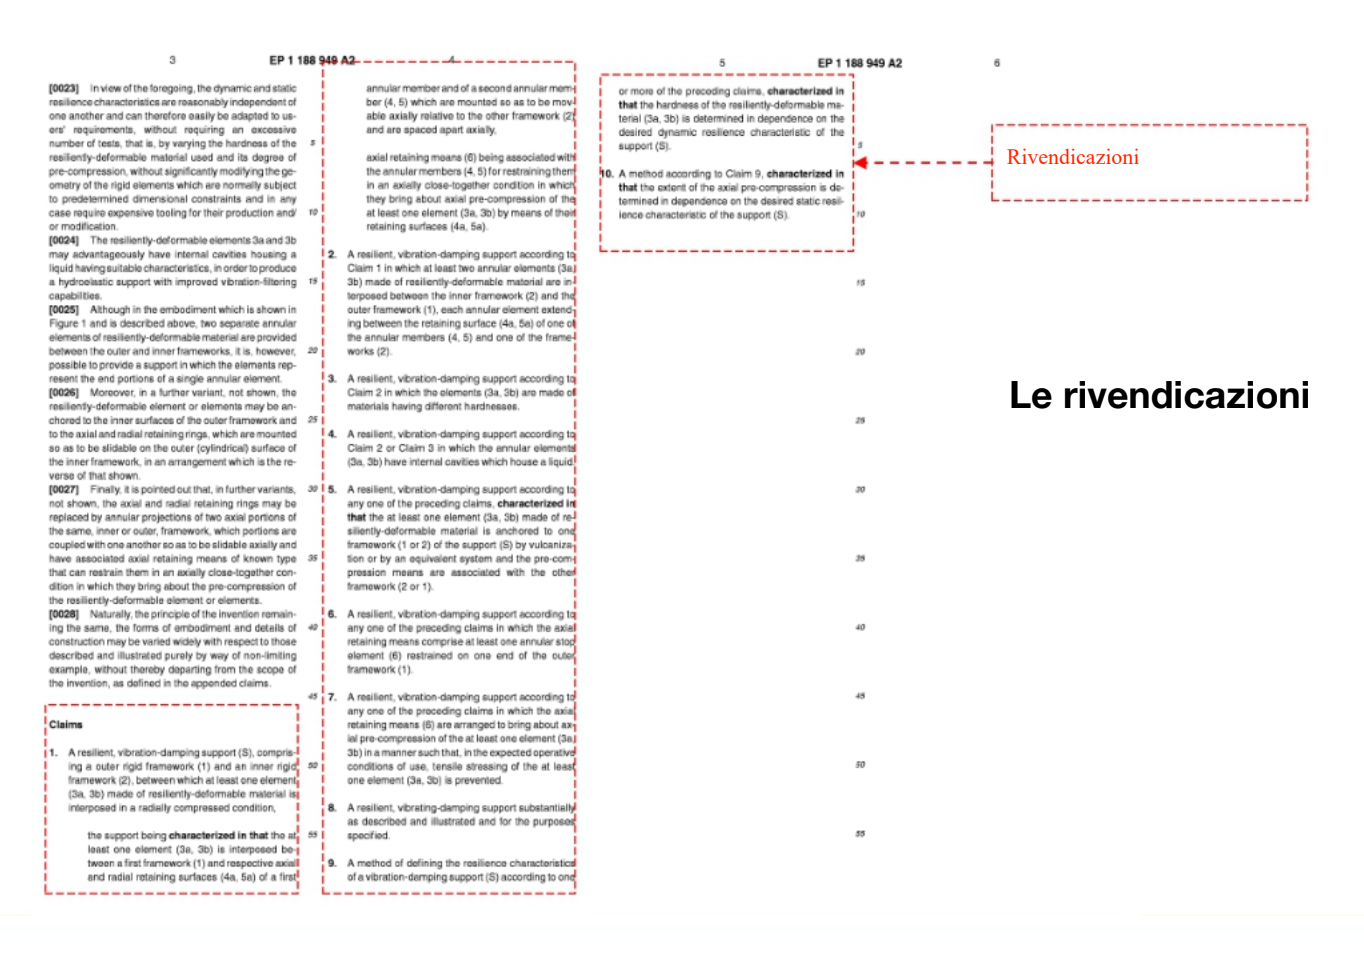
\includegraphics[width=\textwidth]{claims patent.png}
    \caption{Rivendicazioni}
    \label{claims}
\end{figure}

\subsection{Disegni}
Vedi figura \ref{disegni}

\begin{figure}[!]
    \centering
    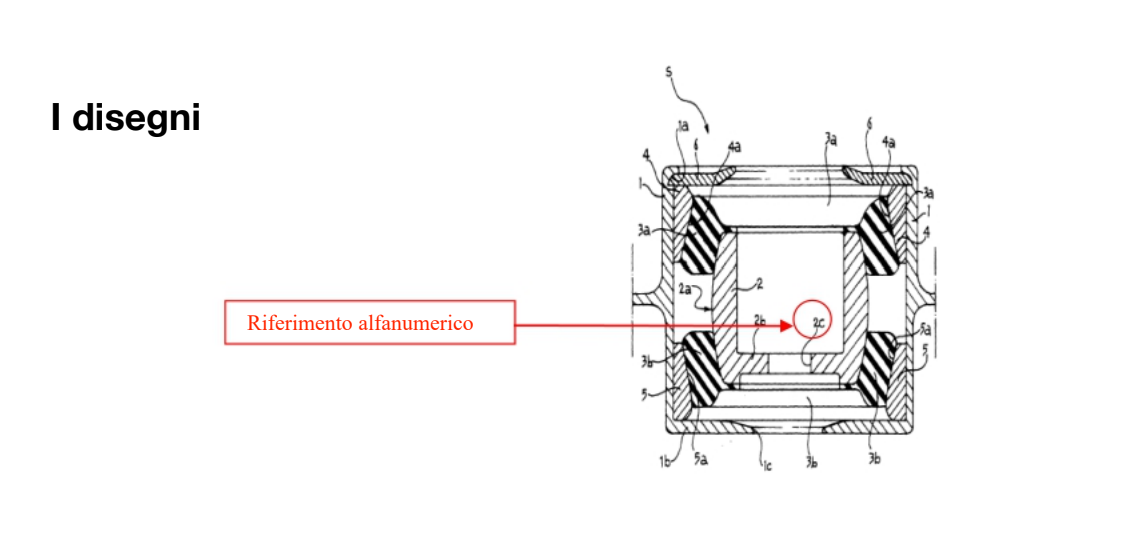
\includegraphics[width=\textwidth]{disegni.png}
    \caption{Disegni}
    \label{disegni}
\end{figure}

\subsection{Rapporto di ricerca}
Vedi figura \ref{rapporto di ricerca}

\begin{figure}[!]
    \centering
    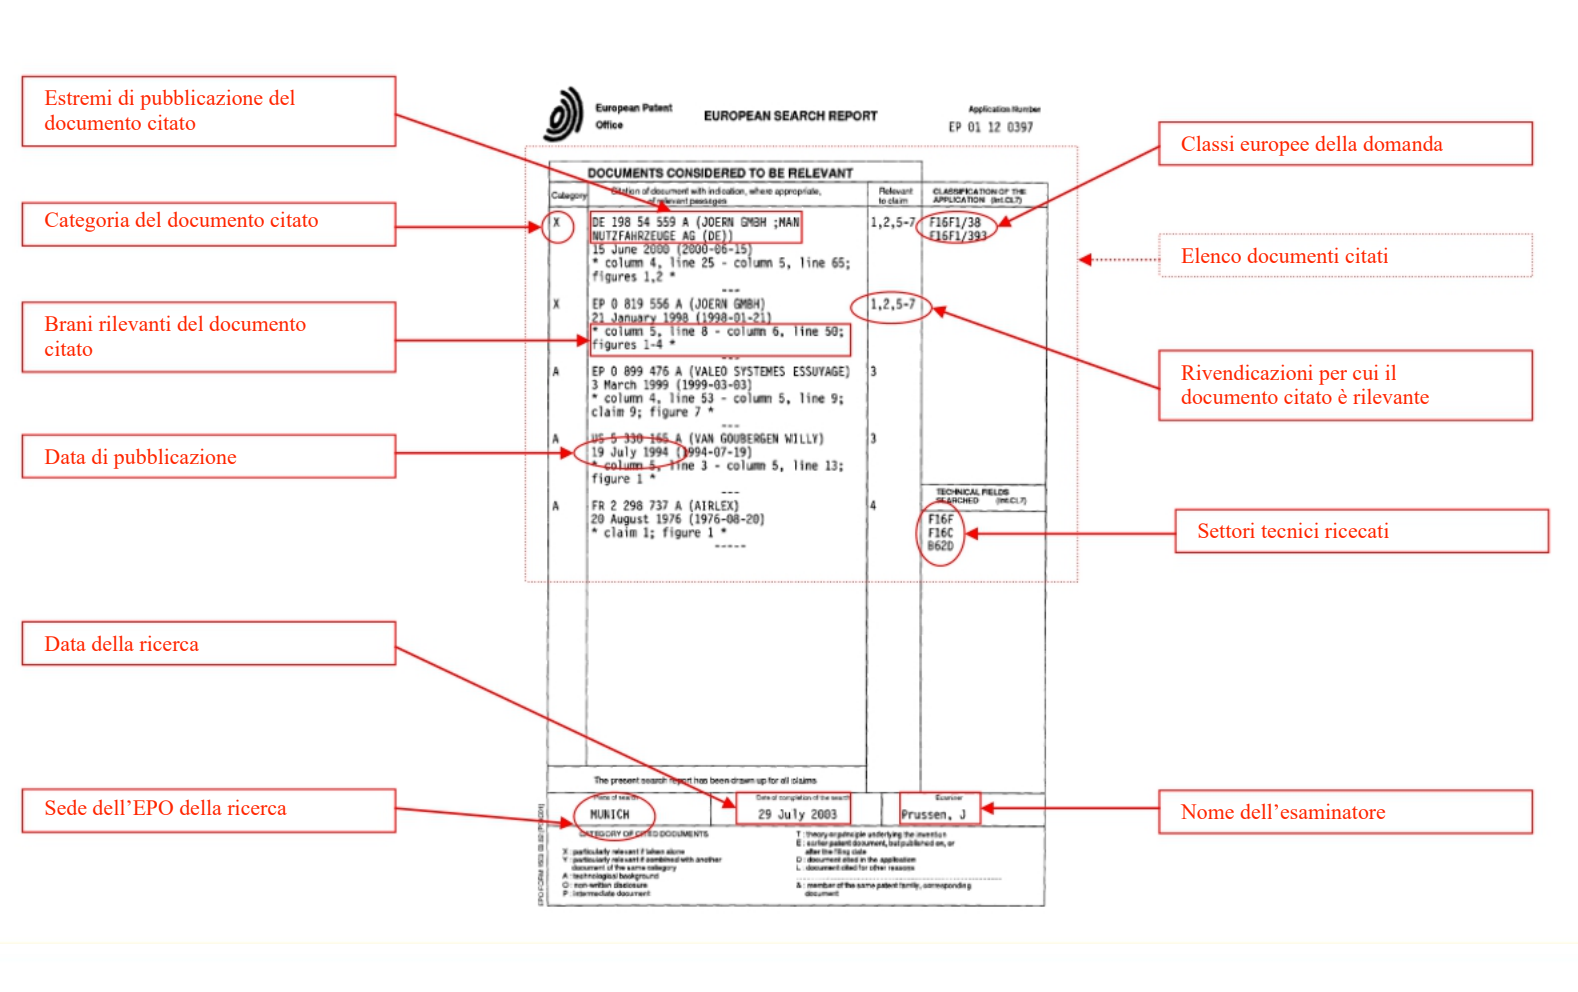
\includegraphics[width=\textwidth]{rapporto di ricerca.png}
    \caption{Rapporto di ricerca}
    \label{rapporto di ricerca}
\end{figure}

